%%% Local Variables:
%%% mode: latex
%%% TeX-master: "<none>"
%%% End:

\label{sec:playing_chunks}

After buffering, the received chunks are sent to the player using a
reliable channel, on demand, starting at the chunk pointed by
$\text{chunk\_to\_play}$, which is incremented one-by-one. Those
chunks that have not been received at the time of sending them to the
player are considered as lost.

\begin{figure*}
  %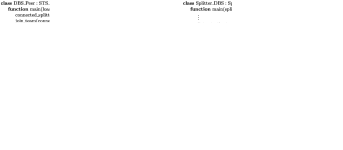
\includegraphics[width=\textwidth]{joining}
  \imgw{1000}{graphics/joining.svg} \caption{Code related to team
    joining.\label{fig:joining}}
\end{figure*}

The new pseudo-code related to joining a team is describen in the
Fig.~\ref{fig:joining}.

